\documentclass[tikz,border=5pt]{standalone}
\usepackage{tikz}
\usetikzlibrary{positioning,calc,shapes.geometric,fit}

\begin{document}
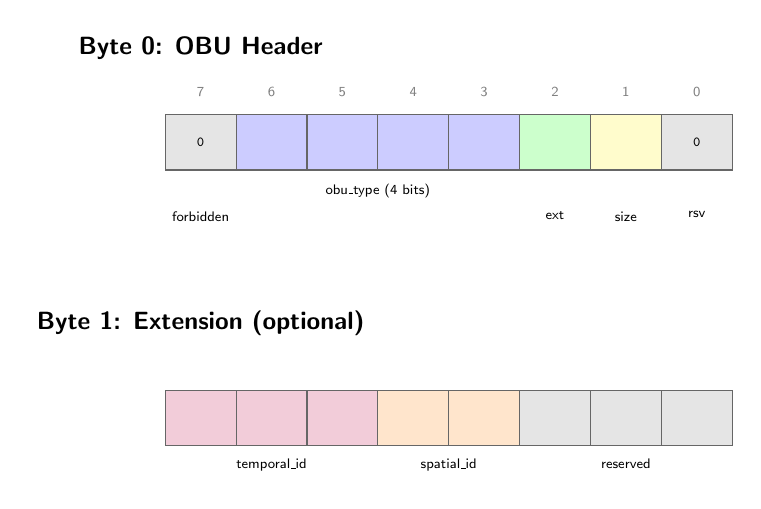
\begin{tikzpicture}[
    bit/.style={draw=black!60, minimum width=0.9cm, minimum height=0.7cm, font=\tiny\ttfamily},
    bitlabel/.style={font=\tiny\sffamily, text=black!50},
    header/.style={font=\small\sffamily\bfseries}
]

% Byte 0: OBU Header
\node[header] at (0, 1.2) {Byte 0: OBU Header};

\node[bit, fill=gray!20] (b7) at (0,0) {0};
\node[bit, fill=blue!20, right=-\pgflinewidth of b7] (b6) {};
\node[bit, fill=blue!20, right=-\pgflinewidth of b6] (b5) {};
\node[bit, fill=blue!20, right=-\pgflinewidth of b5] (b4) {};
\node[bit, fill=blue!20, right=-\pgflinewidth of b4] (b3) {};
\node[bit, fill=green!20, right=-\pgflinewidth of b3] (b2) {};
\node[bit, fill=yellow!20, right=-\pgflinewidth of b2] (b1) {};
\node[bit, fill=gray!20, right=-\pgflinewidth of b1] (b0) {0};

% Bit numbers
\node[bitlabel, above=0.1cm of b7] {7};
\node[bitlabel, above=0.1cm of b6] {6};
\node[bitlabel, above=0.1cm of b5] {5};
\node[bitlabel, above=0.1cm of b4] {4};
\node[bitlabel, above=0.1cm of b3] {3};
\node[bitlabel, above=0.1cm of b2] {2};
\node[bitlabel, above=0.1cm of b1] {1};
\node[bitlabel, above=0.1cm of b0] {0};

% Field labels
\node[below=0.4cm of b7, font=\tiny\sffamily] {forbidden};
\node[below=0.4cm of $(b6)!0.5!(b3)$, font=\tiny\sffamily] {obu\_type (4 bits)};
\node[below=0.4cm of b2, font=\tiny\sffamily] {ext};
\node[below=0.4cm of b1, font=\tiny\sffamily] {size};
\node[below=0.4cm of b0, font=\tiny\sffamily] {rsv};

% Extension header (Byte 1)
\node[header] at (0, -2.3) {Byte 1: Extension (optional)};

\node[bit, fill=purple!20] (e7) at (0,-3.5) {};
\node[bit, fill=purple!20, right=-\pgflinewidth of e7] (e6) {};
\node[bit, fill=purple!20, right=-\pgflinewidth of e6] (e5) {};
\node[bit, fill=orange!20, right=-\pgflinewidth of e5] (e4) {};
\node[bit, fill=orange!20, right=-\pgflinewidth of e4] (e3) {};
\node[bit, fill=gray!20, right=-\pgflinewidth of e3] (e2) {};
\node[bit, fill=gray!20, right=-\pgflinewidth of e2] (e1) {};
\node[bit, fill=gray!20, right=-\pgflinewidth of e1] (e0) {};

\node[below=0.4cm of $(e7)!0.5!(e5)$, font=\tiny\sffamily] {temporal\_id};
\node[below=0.4cm of $(e4)!0.5!(e3)$, font=\tiny\sffamily] {spatial\_id};
\node[below=0.4cm of $(e2)!0.5!(e0)$, font=\tiny\sffamily] {reserved};

\end{tikzpicture}
\end{document}
